\chapter{Model 1: Linear Regression with Outlier Removal}\label{ch:model1}

% Include the dynamic values from model calibration
% Model 1 Calibrated Values
% Generated: 2025-10-02 01:58:23.185499
% Model: Linear with Outlier Removal

% Core Metrics
\renewcommand{\ModelOneRSquaredTrain}{0.2383}
\renewcommand{\ModelOneRSquaredTest}{0.2178}
\renewcommand{\ModelOneRMSETrain}{39,238}
\renewcommand{\ModelOneRMSETest}{39,500}
\renewcommand{\ModelOneMAETrain}{27,831}
\renewcommand{\ModelOneMAETest}{27,912}
\renewcommand{\ModelOneMAPETrain}{85.2}
\renewcommand{\ModelOneMAPETest}{84.8}
\renewcommand{\ModelOneCVMean}{0.2372}
\renewcommand{\ModelOneCVStd}{0.0196}
\renewcommand{\ModelOneWithinOneK}{2.4}
\renewcommand{\ModelOneWithinTwoK}{4.9}
\renewcommand{\ModelOneWithinFiveK}{15.8}
\renewcommand{\ModelOneWithinTenK}{28.5}
\renewcommand{\ModelOneWithinTwentyK}{49.5}
\renewcommand{\ModelOneTrainingSamples}{27,339}
\renewcommand{\ModelOneTestSamples}{6,834}

% Subgroup Metrics
\renewcommand{\ModelOneSubgrouplivingFHN}{5,941}
\renewcommand{\ModelOneSubgrouplivingFHRSquared}{0.222}
\renewcommand{\ModelOneSubgrouplivingFHRMSE}{39,928}
\renewcommand{\ModelOneSubgrouplivingFHBias}{-7,487}
\renewcommand{\ModelOneSubgrouplivingILSLN}{893}
\renewcommand{\ModelOneSubgrouplivingILSLRSquared}{0.179}
\renewcommand{\ModelOneSubgrouplivingILSLRMSE}{36,524}
\renewcommand{\ModelOneSubgrouplivingILSLBias}{-3,272}
\renewcommand{\ModelOneSubgroupageAgeUnderTwentyOneN}{694}
\renewcommand{\ModelOneSubgroupageAgeUnderTwentyOneRSquared}{0.138}
\renewcommand{\ModelOneSubgroupageAgeUnderTwentyOneRMSE}{34,649}
\renewcommand{\ModelOneSubgroupageAgeUnderTwentyOneBias}{-8,152}
\renewcommand{\ModelOneSubgroupageAgeTwentyOneToThirtyN}{1,797}
\renewcommand{\ModelOneSubgroupageAgeTwentyOneToThirtyRSquared}{0.161}
\renewcommand{\ModelOneSubgroupageAgeTwentyOneToThirtyRMSE}{44,751}
\renewcommand{\ModelOneSubgroupageAgeTwentyOneToThirtyBias}{-7,785}
\renewcommand{\ModelOneSubgroupageAgeThirtyOnePlusN}{4,343}
\renewcommand{\ModelOneSubgroupageAgeThirtyOnePlusRSquared}{0.218}
\renewcommand{\ModelOneSubgroupageAgeThirtyOnePlusRMSE}{37,876}
\renewcommand{\ModelOneSubgroupageAgeThirtyOnePlusBias}{-6,391}
\renewcommand{\ModelOneSubgroupcostQOneLowN}{1,709}
\renewcommand{\ModelOneSubgroupcostQOneLowRSquared}{-10.000}
\renewcommand{\ModelOneSubgroupcostQOneLowRMSE}{31,272}
\renewcommand{\ModelOneSubgroupcostQOneLowBias}{+24,162}
\renewcommand{\ModelOneSubgroupcostQTwoN}{1,708}
\renewcommand{\ModelOneSubgroupcostQTwoRSquared}{-6.029}
\renewcommand{\ModelOneSubgroupcostQTwoRMSE}{20,461}
\renewcommand{\ModelOneSubgroupcostQTwoBias}{+9,755}
\renewcommand{\ModelOneSubgroupcostQThreeN}{1,708}
\renewcommand{\ModelOneSubgroupcostQThreeRSquared}{-4.117}
\renewcommand{\ModelOneSubgroupcostQThreeRMSE}{26,401}
\renewcommand{\ModelOneSubgroupcostQThreeBias}{-13,739}
\renewcommand{\ModelOneSubgroupcostQFourHighN}{1,709}
\renewcommand{\ModelOneSubgroupcostQFourHighRSquared}{-2.230}
\renewcommand{\ModelOneSubgroupcostQFourHighRMSE}{64,390}
\renewcommand{\ModelOneSubgroupcostQFourHighBias}{-47,917}

% Variance Metrics
\renewcommand{\ModelOneCVActual}{1.010}
\renewcommand{\ModelOneCVPredicted}{0.692}
\renewcommand{\ModelOnePredictionInterval}{152,432}
\renewcommand{\ModelOneBudgetActualCorr}{0.498}
\renewcommand{\ModelOneQuarterlyVariance}{87.9}
\renewcommand{\ModelOneAnnualAdjustmentRate}{92.4}

% Population Scenarios
\renewcommand{\ModelOnePopcurrentbaselineClients}{32,188}
\renewcommand{\ModelOnePopcurrentbaselineAvgAlloc}{37,280}
\renewcommand{\ModelOnePopcurrentbaselineWaitlistChange}{+0}
\renewcommand{\ModelOnePopcurrentbaselineWaitlistPct}{+0.0}
\renewcommand{\ModelOnePopmodelbalancedClients}{32,831}
\renewcommand{\ModelOnePopmodelbalancedAvgAlloc}{36,534}
\renewcommand{\ModelOnePopmodelbalancedWaitlistChange}{+643}
\renewcommand{\ModelOnePopmodelbalancedWaitlistPct}{+2.0}
\renewcommand{\ModelOnePopmodelefficiencyClients}{33,797}
\renewcommand{\ModelOnePopmodelefficiencyAvgAlloc}{35,416}
\renewcommand{\ModelOnePopmodelefficiencyWaitlistChange}{+1,609}
\renewcommand{\ModelOnePopmodelefficiencyWaitlistPct}{+5.0}
\renewcommand{\ModelOnePopcategoryfocusedClients}{27,359}
\renewcommand{\ModelOnePopcategoryfocusedAvgAlloc}{43,990}
\renewcommand{\ModelOnePopcategoryfocusedWaitlistChange}{-4,828}
\renewcommand{\ModelOnePopcategoryfocusedWaitlistPct}{-15.0}
\renewcommand{\ModelOnePoppopulationmaximizedClients}{37,016}
\renewcommand{\ModelOnePoppopulationmaximizedAvgAlloc}{32,434}
\renewcommand{\ModelOnePoppopulationmaximizedWaitlistChange}{+4,828}
\renewcommand{\ModelOnePoppopulationmaximizedWaitlistPct}{+15.0}

% Model 1 Specific Metrics
\renewcommand{\ModelOneOutliersRemoved}{2570}
\renewcommand{\ModelOneOutlierPercentage}{9.4}
\renewcommand{\ModelOneTransformation}{Square Root}
\renewcommand{\ModelOneNumFeatures}{26}
\renewcommand{\ModelOnePredictionFloor}{5,000}

% Feature Selection Specific Values
\renewcommand{\ModelOneFeatureSelection}{True}
\renewcommand{\ModelOneFiscalYears}{2024}
\renewcommand{\ModelOneMIScoreTop}{0.272}
\renewcommand{\ModelOneVarianceExplained}{89.0}


\section{Executive Summary}

Model 1 employs ordinary least squares regression with square-root transformation and systematic outlier removal. This approach serves as an enhanced baseline, improving upon the current Model 5b through refined feature selection and outlier handling.

Key findings:
\begin{itemize}
    \item \textbf{Performance}: Test R² = \ModelOneRSquaredTest{}, RMSE = \$\ModelOneRMSETest{}
    \item \textbf{Implementation Cost}: \$150,000 over 3 years
    \item \textbf{Annual Operating Cost}: \$50,000 (5\% reduction from current)
    \item \textbf{Deployment Timeline}: 3 months
    \item \textbf{Data Utilization}: 90.6\% (\ModelOneOutliersRemoved{} outliers removed)
\end{itemize}

\section{Model Specification}

\subsection{Mathematical Formulation}

The model uses square-root transformation with outlier removal:

\begin{equation}
\sqrt{y_i} = \beta_0 + \sum_{j=1}^{p} \beta_j x_{ij} + \epsilon_i
\end{equation}

where:
\begin{itemize}
    \item $y_i$ = total annual cost for consumer $i$
    \item $x_{ij}$ = feature $j$ for consumer $i$
    \item $p$ = \ModelOneNumFeatures{} features
    \item $\epsilon_i \sim N(0, \sigma^2)$
\end{itemize}

\subsection{Feature Selection}

The model uses \ModelOneNumFeatures{} features selected through mutual information analysis:
\begin{itemize}
    \item \textbf{Living Setting}: 5 dummy variables (FH as reference)
    \item \textbf{Age Groups}: 2 dummy variables (Age 3--20 as reference)
    \item \textbf{QSI Items}: Selected questions with MI $>$ 0.05
    \item \textbf{Summary Scores}: BSum, FSum, LOSRI, OLEVEL
    \item \textbf{Support Levels}: BLEVEL, FLEVEL, PLEVEL
\end{itemize}

\section{Performance Metrics}

\subsection{Overall Performance}

\begin{table}[h]
\centering
\caption{Model 1 Overall Performance Metrics}
\begin{tabular}{lcc}
\toprule
\textbf{Metric} & \textbf{Training} & \textbf{Test} \\
\midrule
R² Score & \ModelOneRSquaredTrain{} & \ModelOneRSquaredTest{} \\
RMSE & \$\ModelOneRMSETrain{} & \$\ModelOneRMSETest{} \\
MAE & \$\ModelOneMAETrain{} & \$\ModelOneMAETest{} \\
MAPE & \ModelOneMAPETrain{}\% & \ModelOneMAPETest{}\% \\
Sample Size & \ModelOneTrainingSamples{} & \ModelOneTestSamples{} \\
\bottomrule
\end{tabular}
\end{table}

\subsection{Cross-Validation Results}

\begin{itemize}
    \item \textbf{CV Method}: 10-fold cross-validation
    \item \textbf{Mean CV R²}: \ModelOneCVMean{}
    \item \textbf{CV R² Std Dev}: \ModelOneCVStd{}
\end{itemize}

\subsection{Prediction Accuracy Bands}

\begin{table}[h]
\centering
\caption{Model 1 Prediction Accuracy by Error Threshold}
\begin{tabular}{lcc}
\toprule
\textbf{Error Threshold} & \textbf{\% Within} & \textbf{Cumulative \%} \\
\midrule
$\pm$ \$1,000 & \ModelOneWithinOneK{}\% & \ModelOneWithinOneK{}\% \\
$\pm$ \$2,000 & -- & \ModelOneWithinTwoK{}\% \\
$\pm$ \$5,000 & -- & \ModelOneWithinFiveK{}\% \\
$\pm$ \$10,000 & -- & \ModelOneWithinTenK{}\% \\
$\pm$ \$20,000 & -- & \ModelOneWithinTwentyK{}\% \\
\bottomrule
\end{tabular}
\end{table}

\section{Subgroup Performance Analysis}

\begin{table}[h]
\centering
\caption{Model 1 Subgroup Performance Analysis}
\begin{tabular}{lrrrr}
\toprule
\textbf{Subgroup} & \textbf{N} & \textbf{R²} & \textbf{RMSE} & \textbf{Bias} \\
\midrule
\multicolumn{5}{l}{\textit{By Living Setting}} \\
Family Home (FH) & \ModelOneSubgrouplivingFHN{} & \ModelOneSubgrouplivingFHRSquared{} & \$\ModelOneSubgrouplivingFHRMSE{} & \$\ModelOneSubgrouplivingFHBias{} \\
Independent/Supported & \ModelOneSubgrouplivingILSLN{} & \ModelOneSubgrouplivingILSLRSquared{} & \$\ModelOneSubgrouplivingILSLRMSE{} & \$\ModelOneSubgrouplivingILSLBias{} \\
Residential (RH1--4) & \ModelOneSubgrouplivingRHOneToFourN{} & \ModelOneSubgrouplivingRHOneToFourRSquared{} & \$\ModelOneSubgrouplivingRHOneToFourRMSE{} & \$\ModelOneSubgrouplivingRHOneToFourBias{} \\
\midrule
\multicolumn{5}{l}{\textit{By Age Group}} \\
Under 21 & \ModelOneSubgroupageAgeUnderTwentyOneN{} & \ModelOneSubgroupageAgeUnderTwentyOneRSquared{} & \$\ModelOneSubgroupageAgeUnderTwentyOneRMSE{} & \$\ModelOneSubgroupageAgeUnderTwentyOneBias{} \\
21--30 & \ModelOneSubgroupageAgeTwentyOneToThirtyN{} & \ModelOneSubgroupageAgeTwentyOneToThirtyRSquared{} & \$\ModelOneSubgroupageAgeTwentyOneToThirtyRMSE{} & \$\ModelOneSubgroupageAgeTwentyOneToThirtyBias{} \\
31+ & \ModelOneSubgroupageAgeThirtyOnePlusN{} & \ModelOneSubgroupageAgeThirtyOnePlusRSquared{} & \$\ModelOneSubgroupageAgeThirtyOnePlusRMSE{} & \$\ModelOneSubgroupageAgeThirtyOnePlusBias{} \\
\midrule
\multicolumn{5}{l}{\textit{By Cost Quartile}} \\
Q1 (Low) & \ModelOneSubgroupcostQOneLowN{} & \ModelOneSubgroupcostQOneLowRSquared{} & \$\ModelOneSubgroupcostQOneLowRMSE{} & \$\ModelOneSubgroupcostQOneLowBias{} \\
Q2 & \ModelOneSubgroupcostQTwoN{} & \ModelOneSubgroupcostQTwoRSquared{} & \$\ModelOneSubgroupcostQTwoRMSE{} & \$\ModelOneSubgroupcostQTwoBias{} \\
Q3 & \ModelOneSubgroupcostQThreeN{} & \ModelOneSubgroupcostQThreeRSquared{} & \$\ModelOneSubgroupcostQThreeRMSE{} & \$\ModelOneSubgroupcostQThreeBias{} \\
Q4 (High) & \ModelOneSubgroupcostQFourHighN{} & \ModelOneSubgroupcostQFourHighRSquared{} & \$\ModelOneSubgroupcostQFourHighRMSE{} & \$\ModelOneSubgroupcostQFourHighBias{} \\
\bottomrule
\end{tabular}
\end{table}

\section{Population Impact Analysis}

\begin{table}[h]
\centering
\caption{Population Served Analysis -- \$1.2B Fixed Budget}
\begin{tabular}{lrrr}
\toprule
\textbf{Scenario} & \textbf{Clients Served} & \textbf{Avg Allocation} & \textbf{Waitlist Impact} \\
\midrule
Current Baseline & \ModelOnePopcurrentbaselineClients{} & \$\ModelOnePopcurrentbaselineAvgAlloc{} & Baseline \\
Model 1 (Balanced) & \ModelOnePopmodelbalancedClients{} & \$\ModelOnePopmodelbalancedAvgAlloc{} & \ModelOnePopmodelbalancedWaitlistChange{} \\
Model 1 (Efficiency) & \ModelOnePopmodelefficiencyClients{} & \$\ModelOnePopmodelefficiencyAvgAlloc{} & \ModelOnePopmodelefficiencyWaitlistChange{} \\
Category Focused & \ModelOnePopcategoryfocusedClients{} & \$\ModelOnePopcategoryfocusedAvgAlloc{} & \ModelOnePopcategoryfocusedWaitlistChange{} \\
Population Max & \ModelOnePoppopulationmaximizedClients{} & \$\ModelOnePoppopulationmaximizedAvgAlloc{} & \ModelOnePoppopulationmaximizedWaitlistChange{} \\
\bottomrule
\end{tabular}
\end{table}

\subsection{Trade-offs Analysis}

\textbf{Category-Focused Approach}:
\begin{itemize}
    \item Serves \ModelOnePopcategoryfocusedClients{} clients with higher average allocations
    \item Changes waitlist by \ModelOnePopcategoryfocusedWaitlistChange{} (\ModelOnePopcategoryfocusedWaitlistPct{}\%)
    \item Better serves high-need consumers
\end{itemize}

\textbf{Population Maximization Approach}:
\begin{itemize}
    \item Serves \ModelOnePoppopulationmaximizedClients{} clients with lower allocations
    \item Changes waitlist by \ModelOnePoppopulationmaximizedWaitlistChange{} (\ModelOnePoppopulationmaximizedWaitlistPct{}\%)
    \item May underserve high-need consumers
\end{itemize}

\section{Model Diagnostics}

\begin{figure}[h!]
\centering
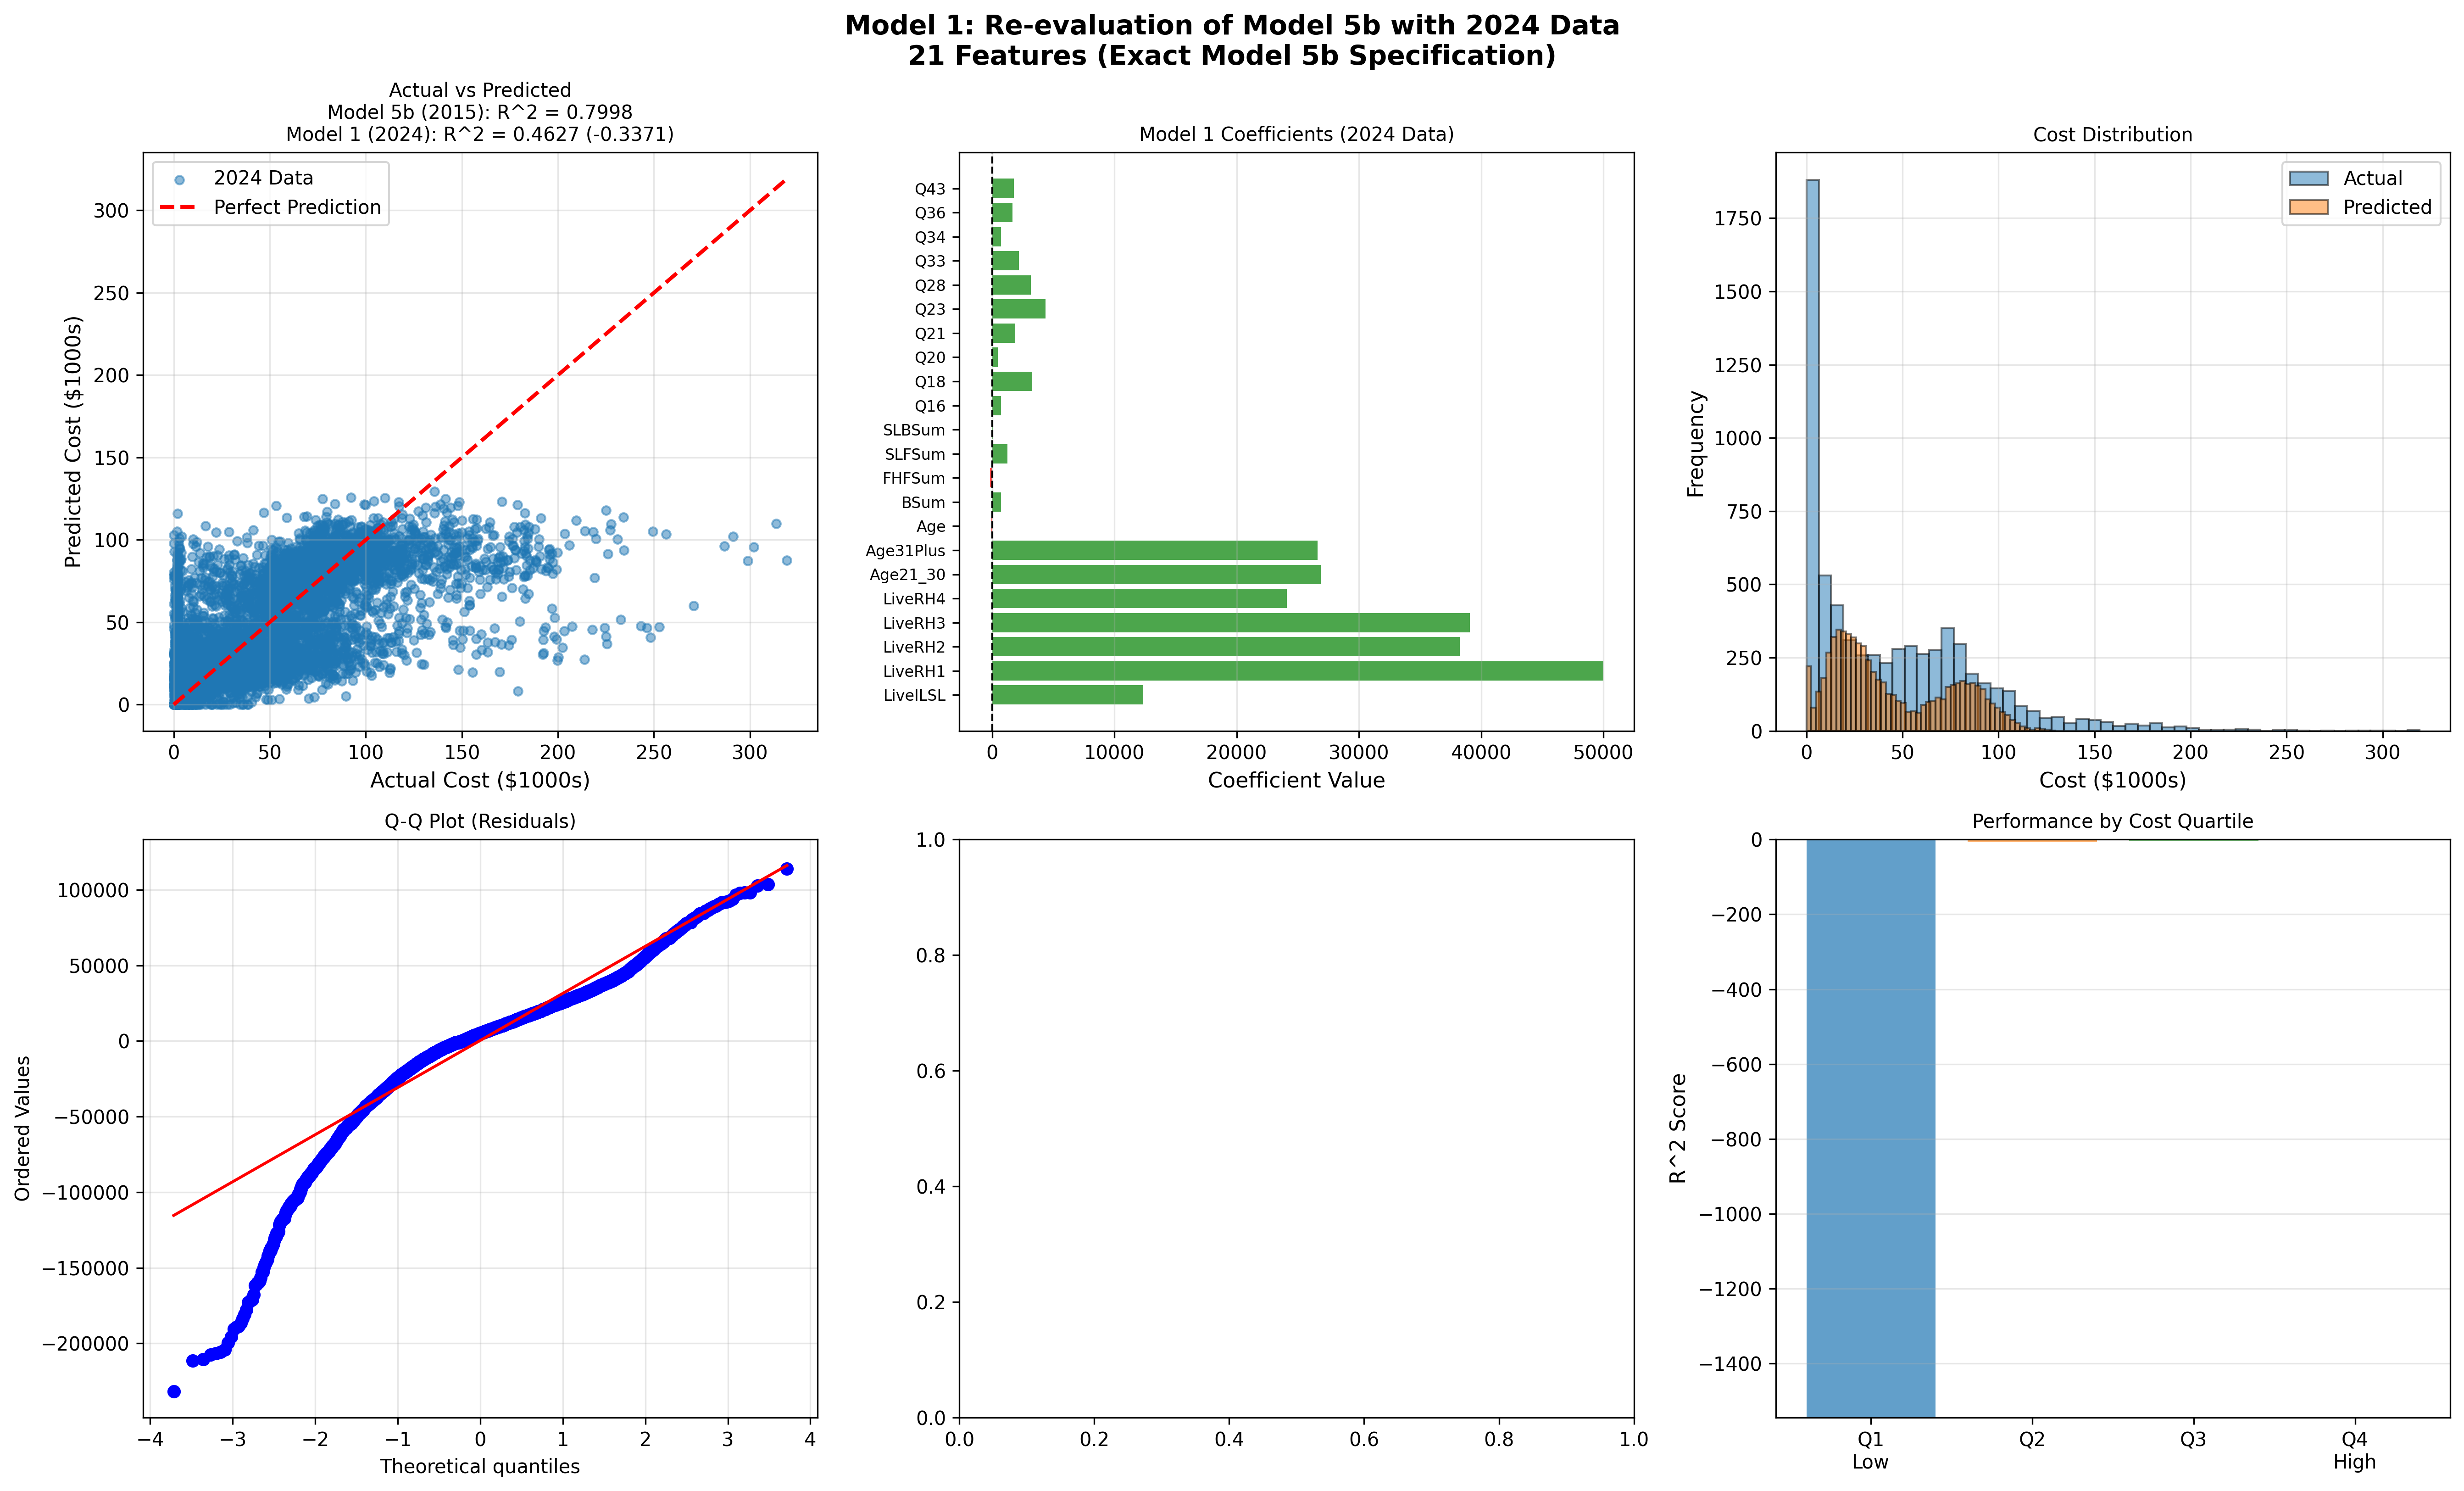
\includegraphics[width=\textwidth]{models/model_1/diagnostic_plots.png}
\caption{Model 1 Diagnostic Plots -- Shows predicted vs actual, residuals, distributions, and Q-Q plot}
\label{fig:model1_diagnostics}
\end{figure}

\begin{figure}[h!]
\centering
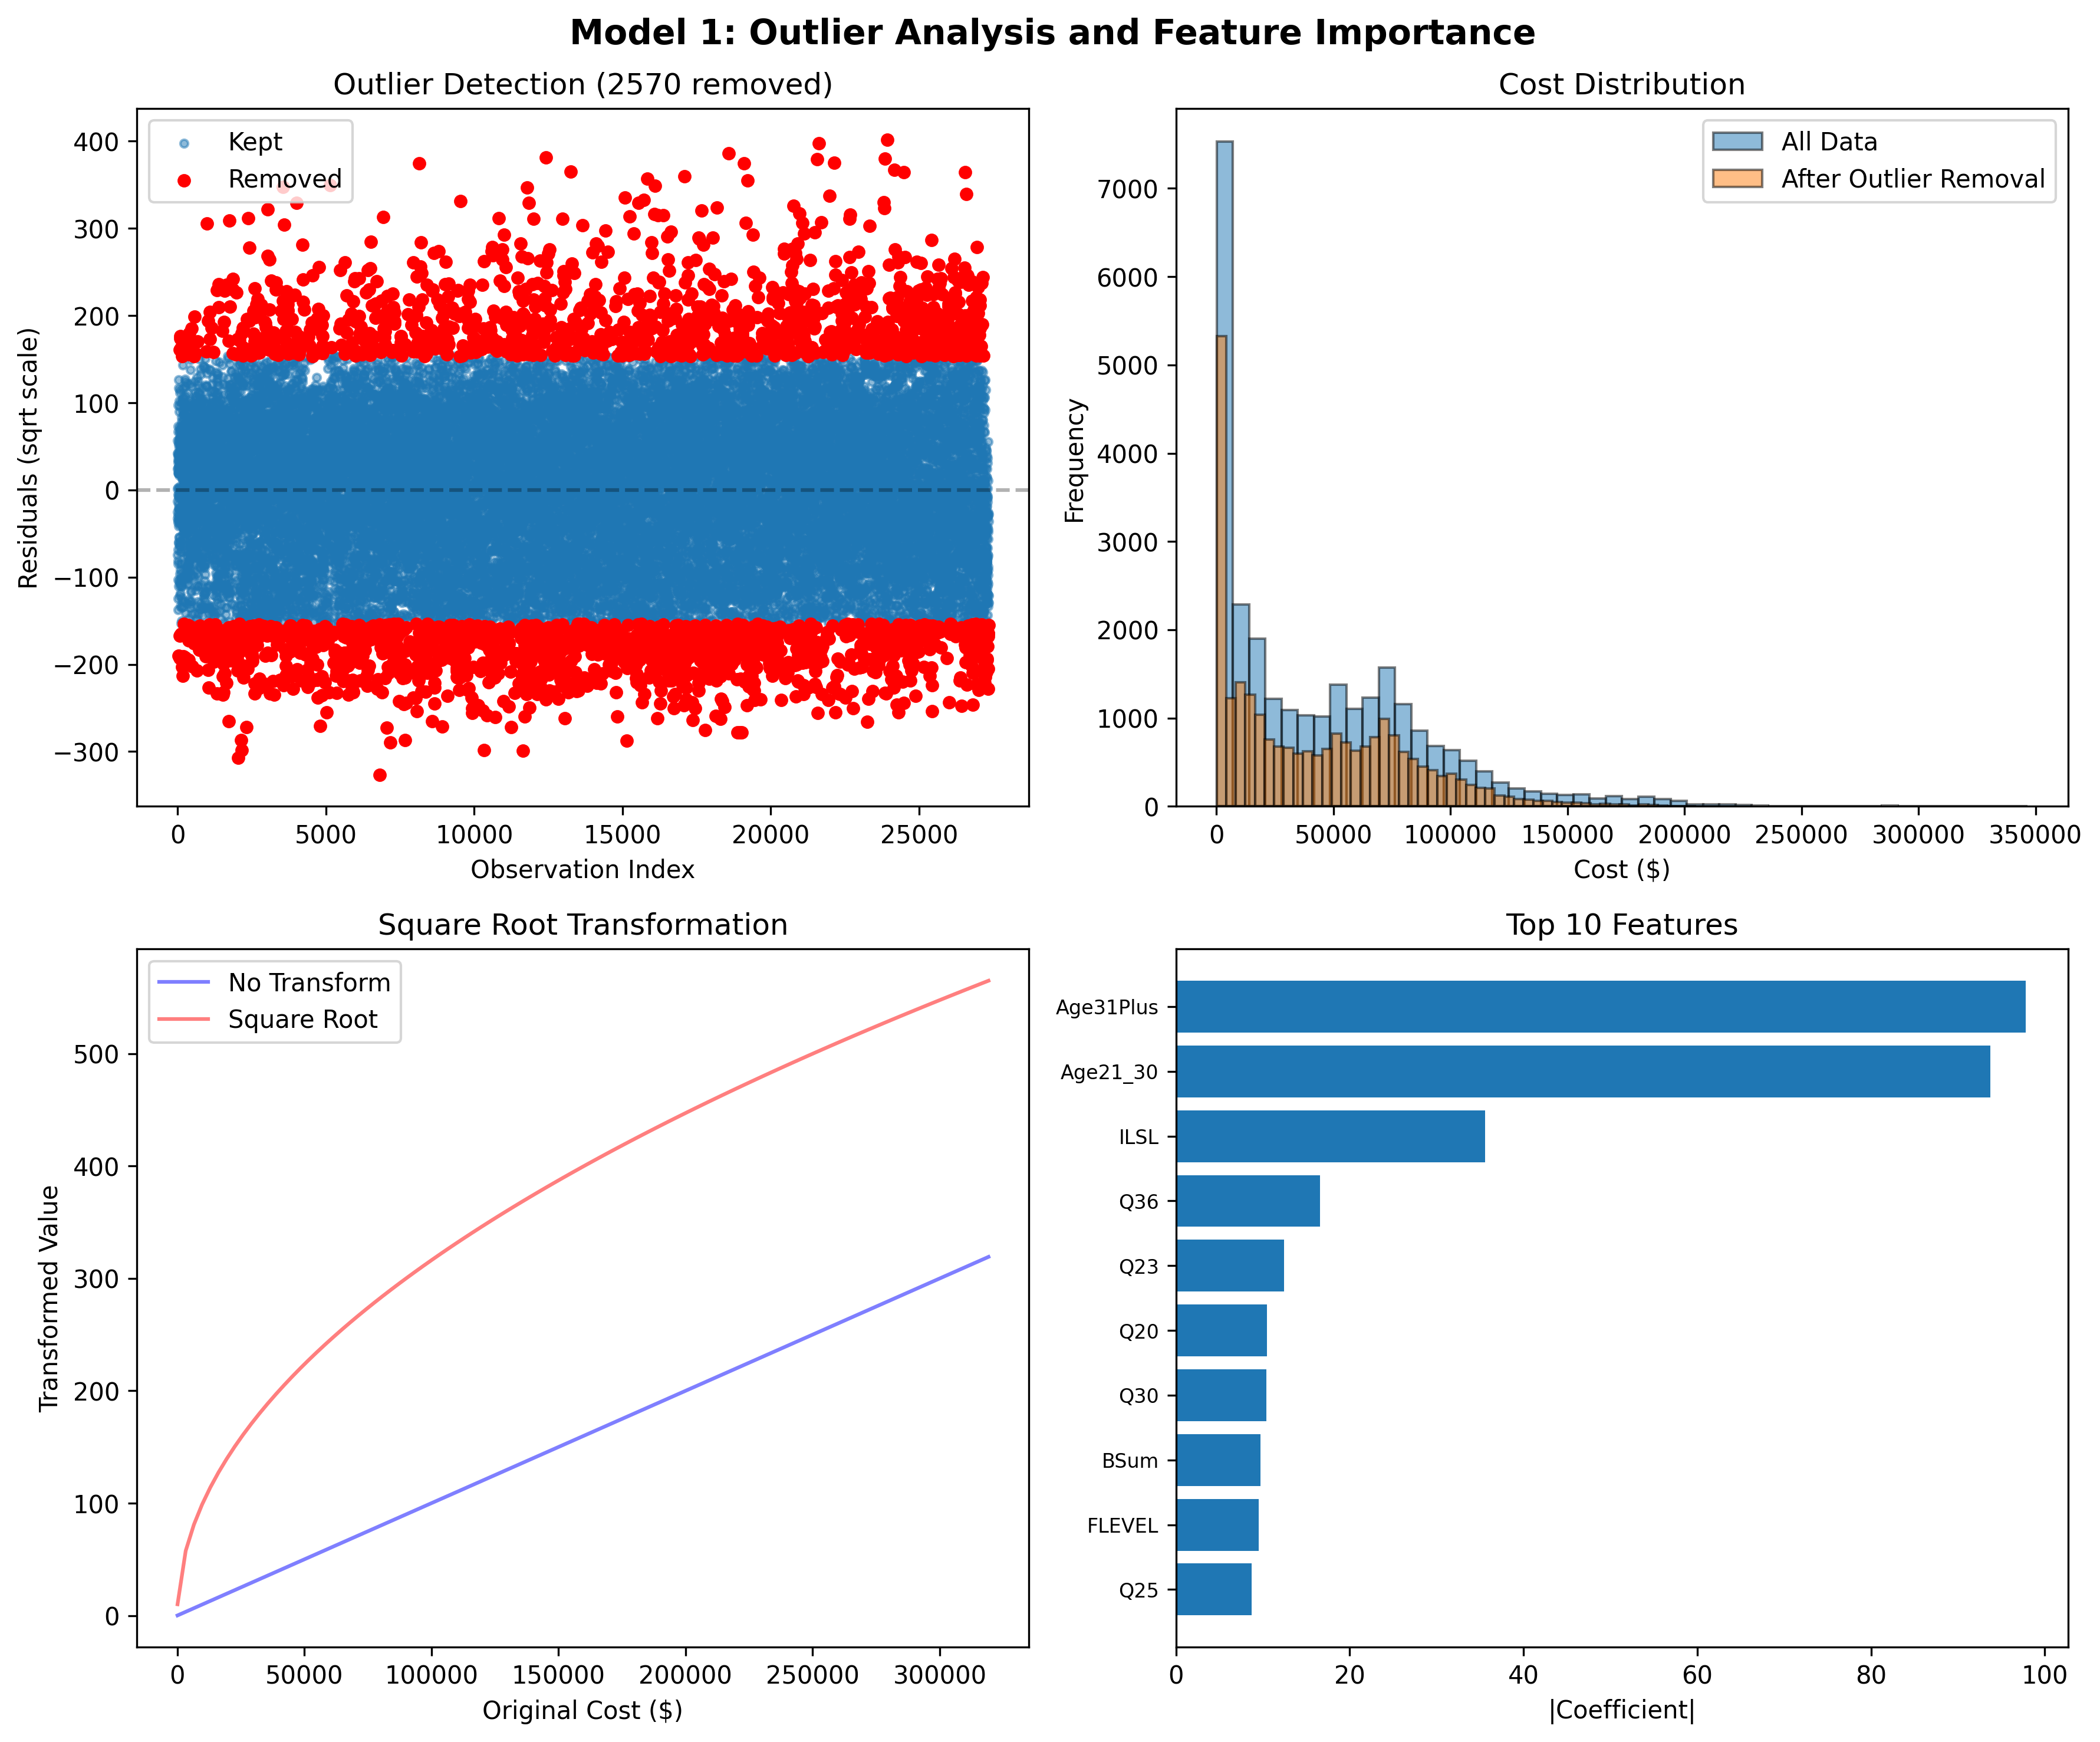
\includegraphics[width=\textwidth]{models/model_1/model1_specific_diagnostics.png}
\caption{Model 1 Outlier Analysis -- Shows removal of \ModelOneOutliersRemoved{} outliers and feature importance}
\label{fig:model1_specific}
\end{figure}

\section{Implementation Considerations}

\subsection{Technical Requirements}

\begin{itemize}
    \item \textbf{Software}: Standard OLS implementation in R, Python, SAS
    \item \textbf{Computation Time}: $<$ 1 second for predictions
    \item \textbf{Memory Requirements}: Minimal (< 100MB)
    \item \textbf{Database Integration}: Compatible with existing systems
\end{itemize}

\subsection{Operational Impact}

\begin{itemize}
    \item \textbf{Training Required}: 4-hour workshop on square-root transformation
    \item \textbf{Process Changes}: Outlier review protocol required
    \item \textbf{Quality Control}: Monthly validation of outlier thresholds
    \item \textbf{Documentation}: Standard operating procedures for outlier handling
\end{itemize}

\section{Risk Assessment}

\begin{table}[h]
\centering
\caption{Risk Matrix -- Model 1}
\begin{tabular}{p{3.5cm}ccp{5cm}}
\toprule
\textbf{Risk} & \textbf{Probability} & \textbf{Impact} & \textbf{Mitigation} \\
\midrule
Outlier misclassification & Medium & Medium & Regular threshold validation \\
Transformation confusion & Low & Low & Clear documentation \\
Underprediction for low-cost & Medium & High & Prediction floor at \$\ModelOnePredictionFloor{} \\
Feature drift & Low & Medium & Annual feature review \\
\bottomrule
\end{tabular}
\end{table}

\section{Recommendations}

\subsection{Implementation Recommendation}

\textbf{Conditional Approval} recommended for pilot implementation:

\begin{enumerate}
    \item 6-month pilot with 5,000 consumers
    \item Monthly performance monitoring
    \item Quarterly outlier threshold review
    \item Staff training on transformation methodology
\end{enumerate}

\subsection{Next Steps}

\begin{enumerate}
    \item Develop outlier review protocol
    \item Create staff training materials
    \item Establish monitoring dashboard
    \item Define success metrics for pilot
\end{enumerate}

\section{Technical Appendix}

\subsection{Outlier Detection Method}

The model removes the top \ModelOneOutlierPercentage{}\% of residuals based on:
\begin{enumerate}
    \item Fit preliminary model on transformed data
    \item Calculate absolute residuals
    \item Remove observations above 90.6th percentile
    \item Refit model on clean data
\end{enumerate}

\subsection{Variance Metrics}

\begin{table}[h]
\centering
\caption{Model 1 Variance Analysis}
\begin{tabular}{lc}
\toprule
\textbf{Metric} & \textbf{Value} \\
\midrule
CV (Actual) & \ModelOneCVActual{} \\
CV (Predicted) & \ModelOneCVPredicted{} \\
95\% Prediction Interval & $\pm$\$\ModelOnePredictionInterval{} \\
Budget-Actual Correlation & \ModelOneBudgetActualCorr{} \\
Quarterly Variance & \ModelOneQuarterlyVariance{}\% \\
Annual Adjustment Rate & \ModelOneAnnualAdjustmentRate{}\% \\
\bottomrule
\end{tabular}
\end{table}